\documentclass[10pt,pscyr,nonums]{hedlab}
\usepackage[russian]{babel}
\usepackage{hedmaths}
\usepackage{graphicx}
\graphicspath{{images/}}
\pagestyle{empty}

\newgeometry{top=1.5cm, bottom=1.5cm, left=1cm, right=1cm}

\student{} \date{}
\labnum{3}
\labname{Исследование статических характеристик триода}

\begin{document}
  \makeheader

  \emph{Цель работы:} изучение методов определения статических характеристик
  триода и изучение режимов его работы.
  
  \begin{figure}[h!]
    \center
    \includegraphics[width=.45\textwidth]{appearance} \hspace*{2em}
    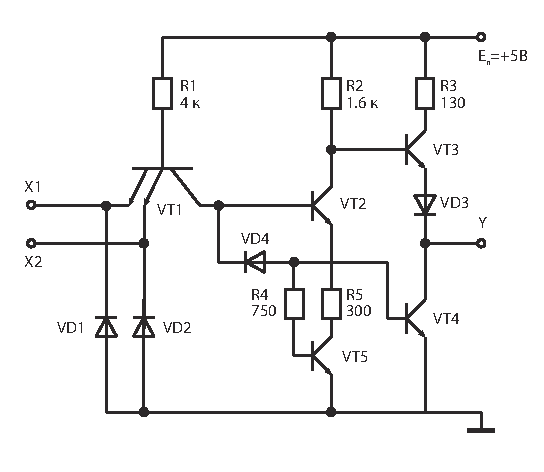
\includegraphics[width=.4\textwidth]{scheme}
    \parbox{.45\textwidth}{\caption{Внешний вид экспериментального макета}}
    \hspace*{2em}
    \parbox{.4\textwidth}{\caption{Принципиальная электрическая схема
    экспериментальной установки}}
  \end{figure}
  
  \begin{table}[h!]
    \center
    \caption{Семейство анодно-сеточных характеристик}
    \begin{tabular}{|m{.1\textwidth}|*{8}{C{.07}|}} \hline
    \multirow{5}{*}{\( U_{a_{01}} =  \)} & \( U_c \),~В &
      &&&&&& \\ \cline{2-9}
    & \( I_{a_1} \),~мА &
      &&&&&& \\ \cline{2-9}
    & \( I_{a_2} \),~мА &
      &&&&&& \\ \cline{2-9}
    & \( I_{a_3} \),~мА &
      &&&&&& \\ \cline{2-9}
    & \( \midnum{I_a} \),~мА &
      &&&&&& \\ \hline
    \multirow{5}{*}{\( U_{a_{02}} = \)} & \( U_c \),~В &
      &&&&&& \\ \cline{2-9}
    & \( I_{a_1} \),~мА &
      &&&&&& \\ \cline{2-9}
    & \( I_{a_2} \),~мА &
      &&&&&& \\ \cline{2-9}
    & \( I_{a_3} \),~мА &
      &&&&&& \\ \cline{2-9}
    & \( \midnum{I_a} \),~мА &
      &&&&&& \\ \hline
    \multirow{5}{*}{\( U_{a_{03}} = \)} & \( U_c \),~В &
      &&&&&& \\ \cline{2-9}
    & \( I_{a_1} \),~мА &
      &&&&&& \\ \cline{2-9}
    & \( I_{a_2} \),~мА &
      &&&&&& \\ \cline{2-9}
    & \( I_{a_3} \),~мА &
      &&&&&& \\ \cline{2-9}
    & \( \midnum{I_a} \),~мА &
      &&&&&& \\ \hline
    \multirow{5}{*}{\( U_{a_{04}} = \)} & \( U_c \),~В &
      &&&&&& \\ \cline{2-9}
    & \( I_{a_1} \),~мА &
      &&&&&& \\ \cline{2-9}
    & \( I_{a_2} \),~мА &
      &&&&&& \\ \cline{2-9}
    & \( I_{a_3} \),~мА &
      &&&&&& \\ \cline{2-9}
    & \( \midnum{I_a} \),~мА &
      &&&&&& \\ \hline
    \end{tabular}
  \end{table}
  
  \pagebreak
  
  \begin{table}[h!]
    \center
    \caption{Семейство анодных характеристик триода}
    \begin{tabular}{|m{.12\textwidth}|C{.07}|*{9}{C{.05}|}} \hline
    \multirow{5}{*}{\( U_{c_{01}} = \)} & \( U_a \),~В &
      &&&&&&&& \\ \cline{2-11}
    & \( I_{a_1} \),~мА &
      &&&&&&&& \\ \cline{2-11}
    & \( I_{a_2} \),~мА &
      &&&&&&&& \\ \cline{2-11}
    & \( I_{a_3} \),~мА &
      &&&&&&&& \\ \cline{2-11}
    & \( \midnum{I_a} \),~мА &
      &&&&&&&& \\ \hline
    \multirow{5}{*}{\( U_{c_{02}} = \)} & \( U_a \),~В &
      &&&&&&&& \\ \cline{2-11}
    & \( I_{a_1} \),~мА &
      &&&&&&&& \\ \cline{2-11}
    & \( I_{a_2} \),~мА &
      &&&&&&&& \\ \cline{2-11}
    & \( I_{a_3} \),~мА &
      &&&&&&&& \\ \cline{2-11}
    & \( \midnum{I_a} \),~мА &
      &&&&&&&& \\ \hline
    \multirow{5}{*}{\( U_{c_{03}} = \)} & \( U_a \),~В &
      &&&&&&&& \\ \cline{2-11}
    & \( I_{a_1} \),~мА &
      &&&&&&&& \\ \cline{2-11}
    & \( I_{a_2} \),~мА &
      &&&&&&&& \\ \cline{2-11}
    & \( I_{a_3} \),~мА &
      &&&&&&&& \\ \cline{2-11}
    & \( \midnum{I_a} \),~мА &
      &&&&&&&& \\ \hline
    \multirow{5}{*}{\( U_{c_{04}} = \)} & \( U_a \),~В &
      &&&&&&&& \\ \cline{2-11}
    & \( I_{a_1} \),~мА &
      &&&&&&&& \\ \cline{2-11}
    & \( I_{a_2} \),~мА &
      &&&&&&&& \\ \cline{2-11}
    & \( I_{a_3} \),~мА &
      &&&&&&&& \\ \cline{2-11}
    & \( \midnum{I_a} \),~мА &
      &&&&&&&& \\ \hline
    \multirow{5}{*}{\( U_{c_{05}} = \)} & \( U_a \),~В &
      &&&&&&&& \\ \cline{2-11}
    & \( I_{a_1} \),~мА &
      &&&&&&&& \\ \cline{2-11}
    & \( I_{a_2} \),~мА &
      &&&&&&&& \\ \cline{2-11}
    & \( I_{a_3} \),~мА &
      &&&&&&&& \\ \cline{2-11}
    & \( \midnum{I_a} \),~мА &
      &&&&&&&& \\ \hline
    \end{tabular}
  \end{table}
\end{document}
